\chapter{Long Context, Retrieval, and Memory}
\label{ch:long-context-retrieval-memory}
\raggedbottom

In 2024, a simple benchmark called needle-in-a-haystack became a standard demo for long-context models: hide one sentence inside a long document, ask for it, and see whether the model can find it. Some models performed impressively. But RULER showed why that demo was too easy: searching for one literal needle says little about multi-hop tracing, aggregation, or robustness as context length grows~\cite{hsieh2024ruler}. NoLiMa pushed the point further by removing direct lexical overlap between the question and the evidence, forcing the model to locate information by association rather than by string matching~\cite{modarressi2025nolima}.

This is the central lesson of context systems. A million-token window is useful, but it is not the same thing as reliable evidence use. A retrieval system is useful, but it is not the opposite of long context. A memory store is useful, but it can also preserve obsolete or private information. Modern model systems must decide which tokens deserve to enter the model at runtime.

Chapter~\ref{ch:serving-quantization-cost} treated context as a serving resource: long prompts increase prefill work, KV-cache memory, latency, and cost. This chapter treats context as an information resource:

\begin{quote}
Which evidence should the model see, in what form, at what cost, and with what audit trail?
\end{quote}

\paragraph{Chapter thesis.} \emph{Long context is not the end of RAG; RAG is not the opposite of long context. Modern context systems route, retrieve, cache, compress, and cite information so that the model sees the right evidence at the right time.}

\paragraph{Running example.} Suppose your Project~4 research assistant answers questions about a semester-long capstone project. The relevant information is scattered across papers, experiment logs, code comments, meeting notes, and earlier conversations. Some questions are easy: ``What dataset did we use for the first experiment?'' Some require synthesis: ``Why did the model improve after we changed the data filter?'' Some require recency: ``Which result superseded the failed run from last week?'' A plain assistant may answer from parametric memory. A long-context assistant may paste everything into one prompt. A RAG assistant may retrieve a few chunks. A cached assistant may reuse a stable project corpus. A robust context system chooses among these paths instead of treating every query the same.

\subsection*{Learning Objectives}

After completing this chapter, you should be able to:

\begin{enumerate}
  \item Explain why context is a scarce runtime resource, not merely a larger input field.
  \item Distinguish long-context reading, retrieval-augmented generation, cached context, compression, and persistent memory.
  \item Describe a RAG system in terms of access, selection, and attribution rather than vector database plumbing.
  \item Reason about routing between direct answering, read-all context, retrieve-then-read, cache-then-read, and hybrid paths.
  \item Identify when compression improves cost and when it destroys the only evidence that matters.
  \item Separate persistent memory across sessions from the agent scratchpad and step state studied in Chapter~\ref{ch:tool-use-agent-loops}.
  \item Diagnose context failures using retrieval ablations, oracle retrieval, evidence shuffling, distractors, and citation audits.
\end{enumerate}

\subsection*{Notation}

\begin{center}
\begin{tabularx}{\textwidth}{@{}lX@{}}
\toprule
Symbol & Meaning \\
\midrule
$C$ & Effective context budget available for one model call \\
$D$ & External document or memory collection \\
$q$ & User query or rewritten retrieval query \\
$R_k(q)$ & Top-$k$ retrieved evidence units for query $q$ \\
$s_i$ & Score assigned to candidate evidence unit $i$ by a retriever or reranker \\
$E$ & Evidence actually packed into the prompt \\
$A$ & Generated answer \\
$M$ & Persistent memory store across turns or sessions \\
\bottomrule
\end{tabularx}
\end{center}

\subsection*{Timeline of Key Contributions}

\begin{center}
\begin{tabularx}{\textwidth}{@{}lX@{}}
\toprule
\textbf{Year} & \textbf{Milestone} \\
\midrule
1990s--2000s & BM25 becomes a durable sparse retrieval baseline; later surveys standardize its role in probabilistic relevance models and search systems~\cite{robertson2009probabilistic}. \\
2020 & Dense Passage Retrieval shows that learned dense retrievers can retrieve open-domain evidence for question answering~\cite{karpukhin2020dpr}. \\
2020 & Retrieval-Augmented Generation combines parametric generation with retrieved non-parametric memory~\cite{lewis2020rag}. \\
2023 & Lost-in-the-middle experiments show that models often use evidence less reliably when it appears in the middle of a long context~\cite{liu2023lost}. \\
2024 & RULER expands long-context evaluation beyond vanilla needle-in-a-haystack retrieval~\cite{hsieh2024ruler}. \\
2024 & LongRAG studies longer retrieval units and long-context readers as a hybrid RAG design~\cite{jiang2024longrag}. \\
2024 & Self-Route compares RAG and long-context routing under performance and cost constraints~\cite{li2024raglongcontext}. \\
2025 & NoLiMa evaluates long-context retrieval without direct lexical overlap between query and evidence~\cite{modarressi2025nolima}. \\
2025 & Native Sparse Attention illustrates a broader trend toward selective, hardware-aware long-context computation~\cite{yuan2025nsa}. \\
2026 & DeepSeek-V4 makes million-token context a systems case study in compressed attention, KV-cache economics, and serving-runtime support~\cite{deepseek2026v4release,deepseek2026v4hf,vllm2026deepseekv4}. \\
\bottomrule
\end{tabularx}
\end{center}

\paragraph{What this chapter covers.} We begin by defining the context problem: window size, serving cost, and attention quality. We then treat long context as a system primitive rather than an architecture survey. The middle of the chapter reframes RAG as a three-layer system--access, selection, and attribution--and then studies hybrid context routing: when to answer directly, read everything, retrieve a subset, reuse cached context, or combine retrieval with a long-context reader. The final sections cover compression, memory across sessions, and diagnostics for failures that look like ``hallucination'' but actually begin with evidence selection.


%----------------------------------------------------------------------
\section{The Context Problem: Window, Cost, and Attention Quality}
\label{sec:ch20-context-problem}

The simplest view of context is syntactic: the context window is the maximum number of tokens the model can condition on. That definition is necessary, but it is not enough for systems work. A context window is also a budget. It consumes prefill time, KV-cache memory, and attention bandwidth. It determines which evidence is visible and which evidence is invisible. It shapes what the model can cite, what it can ignore, and what it may overfit to inside the prompt.

In the research-assistant example, the system might have a 200K-token model and a project folder that contains 3 million tokens. Even if the model can technically accept a long prompt, the system still has to decide whether to paste a full paper, a few sections, a summary, retrieved snippets, old meeting notes, or a cached project brief. The user experiences one answer. The runtime makes an evidence-allocation decision.

\subsection{Long Windows Do Not Guarantee Long-Context Understanding}

Long-context models expand what can be shown to the model. They do not guarantee that the model will use every token equally well. Liu et al.\ showed that models can be more accurate when relevant information appears near the beginning or end of the context than when it appears in the middle~\cite{liu2023lost}. RULER showed that near-perfect vanilla needle retrieval does not imply robust long-context behavior on harder retrieval, tracing, and aggregation tasks~\cite{hsieh2024ruler}. NoLiMa makes the same point from another angle: if the question does not share words with the evidence, the task becomes less like string search and more like semantic evidence use~\cite{modarressi2025nolima}.

The lesson is not that long-context models are weak. The lesson is that window length is an upper bound on visibility, not a guarantee of salience. A system that stuffs all documents into the prompt may still fail because the key paragraph is buried, contradicted, stale, or phrased differently from the question.

\subsection{The Serving Cost of More Context}

Chapter~\ref{ch:serving-quantization-cost} separated prompt prefill from per-token decode. Long context stresses three coupled parts of the serving path: prefill work before the first token, KV-cache memory during generation, and per-token attention cost during decode. Architectures such as compressed or sparse attention try to weaken this coupling, but a larger visible context is never free. Context decisions are therefore latency decisions.

A useful accounting identity is:

\[
C_{\text{used}} = C_{\text{system}} + C_{\text{task}} + C_{\text{evidence}} + C_{\text{history}} + C_{\text{output reserve}}.
\]

Only part of the window is available for evidence. The system prompt, tool instructions, user request, conversation history, and expected output length all compete with documents. A context system is the part of the application that manages this competition.

\begin{tcolorbox}[colback=blue!5, colframe=blue!40, title=\textbf{Long Context Does Not Mean Unlimited Attention}]
A larger window changes the feasible set: the system can show the model more evidence. It does not remove the need to choose. The model may attend weakly to middle evidence, get distracted by irrelevant passages, or use stale context over newer evidence. The design problem moves from ``can this fit?'' to ``is this the right evidence to fit?''
\end{tcolorbox}

\begin{figure}[t]
\centering
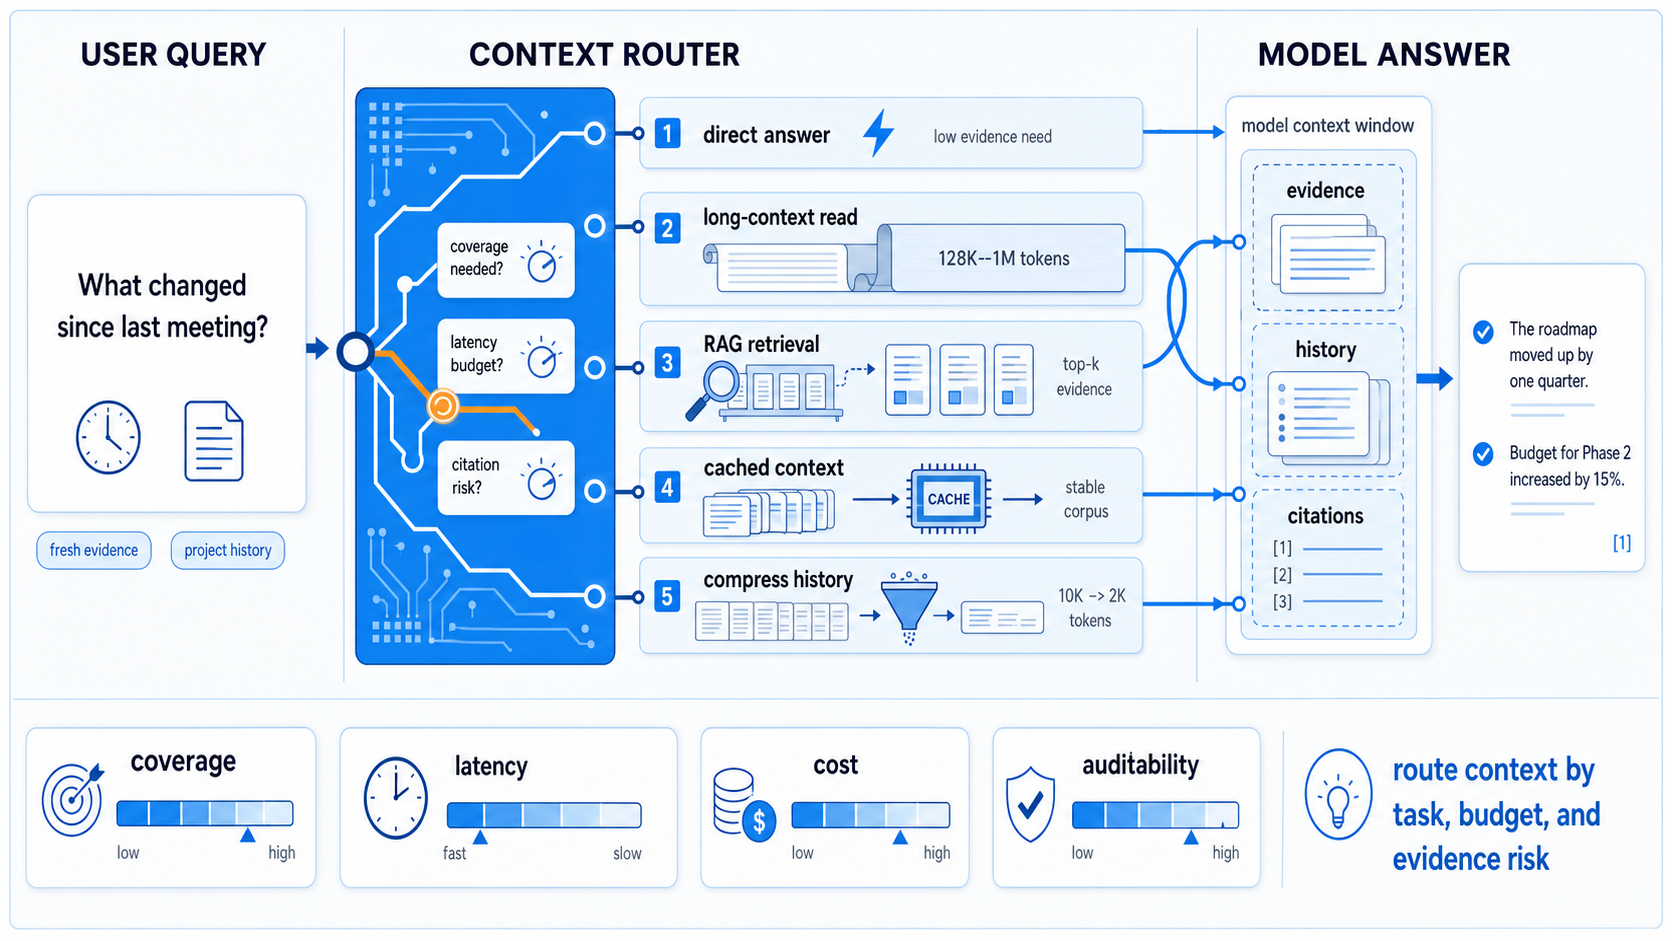
\includegraphics[width=0.96\textwidth]{figures/ch20/fig_context_paths.png}
\caption{\textbf{Context paths for one query.} A context system can answer directly, read a long prompt, retrieve evidence, reuse cached context, compress history, or route to a hybrid path. The chapter's central question is not which path is universally best, but which path fits the task, cost budget, and evidence risk.}
\label{fig:ch20-context-paths}
\end{figure}

\begin{quickrecap}
\textbf{Quick Recap.}
\begin{itemize}[nosep,leftmargin=1.5em]
  \item Context is a runtime resource: it consumes tokens, latency, memory, and attention.
  \item Long windows increase visibility but do not guarantee salience or faithful evidence use.
  \item Needle-in-a-haystack success is not the same as robust long-context understanding.
\end{itemize}
\end{quickrecap}


%----------------------------------------------------------------------
\section{Long Context as a System Primitive}
\label{sec:ch20-long-context-primitive}

This chapter does not teach long-context Transformer architecture in detail. Earlier chapters introduced attention and positional encodings; Chapter~\ref{ch:serving-quantization-cost} explained KV-cache cost. Here the important question is different: once long context exists, how does it change application design?

\subsection{Read-All Context}

The first design pattern is \textbf{read-all context}: place the relevant corpus directly into the prompt and let the model answer from it. This can be the right choice when the corpus is small enough, stable enough, and legally safe to expose to the model call. It avoids retrieval misses because the system does not have to guess which chunk matters.

Read-all context is attractive for the capstone assistant when the user asks about a single 20-page report or a compact experiment log. It is less attractive when the project folder contains months of logs, many near-duplicate drafts, and access-controlled notes. Then ``read all'' becomes expensive and potentially confusing.

\subsection{Long-Context Readers}

Long context also changes the division of labor between retriever and reader. Traditional RAG often retrieves short chunks, so the retriever must locate a small unit precisely and the reader sees only a narrow evidence window. LongRAG argues for longer retrieval units and long-context readers: retrieve fewer, larger units, then let the reader use the surrounding context~\cite{jiang2024longrag}. This moves some burden from exact retrieval to robust reading.

The design tradeoff is clear. Short chunks increase retriever precision but can lose local context. Long units preserve context but risk packing distractors. Neither choice is universally correct. The unit of retrieval should match the unit of reasoning.

\subsection{Caching Stable Context}

If the same large context is reused across many requests, caching becomes a context primitive. Commercial APIs increasingly expose context caching or prompt caching, where a stable prefix or corpus can be stored and referenced in later calls rather than resent each time~\cite{google2026contextcaching}. This changes the cost equation for small, stable corpora. A project brief, documentation bundle, or policy manual may be expensive to load once but cheap to reuse.

Cache-augmented generation is best understood as one route in the context system, not as a replacement for retrieval. It fits stable, repeated, permission-consistent corpora. It is weaker when the corpus changes frequently, when evidence must be selected and cited per answer, or when the corpus is too large to cache as one useful context.

This is also the boundary between caching and memory. Caching reuses already-chosen context to reduce runtime cost. Memory stores information that may be written, retrieved, updated, or forgotten across interactions. A cache is primarily a serving optimization; memory is an information-management policy.

\subsection{Case Study: DeepSeek-V4 and Million-Token Context}

Long-context research is moving toward selective computation. Native Sparse Attention, for example, combines coarse-grained compression with fine-grained token selection to make long-context modeling more efficient on hardware~\cite{yuan2025nsa}. DeepSeek-V4 is a useful 2026 case study because it turns that trend into a full systems example: the official release describes a one-million-token context as a default service capability, with V4-Pro at 1.6T total parameters and 49B activated parameters, and V4-Flash at 284B total parameters and 13B activated parameters~\cite{deepseek2026v4release,deepseek2026v4hf}.

\paragraph{Bottleneck.} A million-token context window is not useful if each decode step must attend densely to a million positions and store a full-resolution KV cache for all of them. That is the direct connection to Chapter~\ref{ch:serving-quantization-cost}: long context is partly a KV-cache and decode-cost problem. vLLM's implementation note frames the main bottlenecks as KV-cache memory growth and attention computation cost, not merely as the ability to declare a larger maximum context length~\cite{vllm2026deepseekv4}.

\paragraph{Compressed sparse and heavily compressed attention.} DeepSeek-V4 combines Compressed Sparse Attention (CSA) and Heavily Compressed Attention (HCA)~\cite{deepseek2026v4hf,deepseek2026v4hfblog}. CSA compresses token-wise KV entries, then uses a lightweight indexer to select relevant compressed blocks. HCA compresses much more aggressively and attends densely over the shorter compressed stream. A short local sliding window preserves high-resolution access to recent tokens before they cross a compression boundary~\cite{vllm2026deepseekv4}. The design lesson is simple: distant information can be compressed and sparsely accessed, while recent local information often needs higher resolution.

\paragraph{Mixed-precision KV cache.} The same case study also shows why long-context design now overlaps with serving quantization. The model card reports that, in the one-million-token setting, V4-Pro uses 27\% of the single-token inference FLOPs and 10\% of the KV cache of a DeepSeek-V3.2 comparison point~\cite{deepseek2026v4hf}. The Hugging Face blog describes FP8 storage for most KV entries, BF16 for RoPE-related dimensions, and FP4 for the CSA indexer~\cite{deepseek2026v4hfblog}. vLLM gives a concrete serving number: with BF16 KV cache, DeepSeek-V4 is estimated at about 9.62 GiB per sequence at one million tokens, compared with an 83.9 GiB estimate for a 61-layer DeepSeek-V3.2-style stack; the deployed FP4/FP8 cache choices reduce memory further~\cite{vllm2026deepseekv4}.

\paragraph{Serving runtime.} Designing the attention pattern is not the end of the story. vLLM reports that supporting DeepSeek-V4 requires managing heterogeneous KV state: some layers use different compression rates, some use sliding-window attention, and batched sequences may sit at different compression boundaries~\cite{vllm2026deepseekv4}. Its implementation uses a shared logical block size, treats compressor state like sliding-window KV, unifies page sizes to reduce fragmentation, and uses kernel fusion and multi-stream execution to reduce decode-path overhead~\cite{vllm2026deepseekv4}. This is the systems punchline: long context is not only a model feature. Architecture, quantization, cache layout, scheduling, and kernels have to agree.

DeepSeek-V4 also includes agent-facing features such as tool-call formats and long-running traces, but those belong to Chapter~\ref{ch:tool-use-agent-loops}. Here the takeaway is narrower: long context has become a managed substrate. The model, KV cache, runtime, and retrieval system together decide what information can be used at task time.

\begin{tcolorbox}[colback=blue!5, colframe=blue!40, title=\textbf{What DeepSeek-V4 Does Not Prove}]
DeepSeek-V4 shows that million-token context can be made more economically usable. It does not show that million-token evidence use is automatically reliable. The system still needs routing, retrieval, compression, attribution, and diagnostics. Efficient access to many tokens is not the same as faithful use of the right tokens.
\end{tcolorbox}

\begin{tcolorbox}[colback=gray!8, colframe=gray!40, title=\textbf{Echo from Ch19: Context Is Part of the Cost Model}]
Chapter~\ref{ch:serving-quantization-cost} measured serving quality with TTFT, TPOT, memory, and cost per useful task. Ch20 applies the same discipline to evidence. A context path that improves accuracy but doubles latency may be right for research analysis and wrong for interactive chat. A path that is cheap but misses the only relevant evidence is not cheap in task-success terms.
\end{tcolorbox}

\begin{quickrecap}
\textbf{Quick Recap.}
\begin{itemize}[nosep,leftmargin=1.5em]
  \item Long context enables read-all prompts, long readers, and cached corpora.
  \item Long retrieval units trade precise retrieval for richer local evidence.
  \item Caching helps stable repeated context, but dynamic or auditable corpora still need selection.
  \item DeepSeek-V4 illustrates the 2026 long-context pattern: efficient long context requires compressed or sparse attention, KV-cache compression, locality preservation, and serving-runtime support.
\end{itemize}
\end{quickrecap}


%----------------------------------------------------------------------
\section{Retrieval-Augmented Generation: Access, Selection, and Attribution}
\label{sec:ch20-rag-access-selection-attribution}

Retrieval-augmented generation (RAG) is often described as a vector database pattern. That framing is too narrow. RAG is a way of turning an external information collection into usable context for a model call~\cite{lewis2020rag}. It has three conceptual layers:

\begin{enumerate}[nosep]
  \item \textbf{Access}: find candidate evidence that might be relevant.
  \item \textbf{Selection}: choose and order the evidence most likely to help.
  \item \textbf{Attribution}: connect generated claims back to supporting sources.
\end{enumerate}

These layers are more important than any particular tool. A system can use BM25, dense embeddings, hybrid retrieval, rerankers, or metadata filters. The central question is whether the answer is grounded in evidence that was actually retrieved, selected, and cited.

\subsection{Access: Can the System Find Candidate Evidence?}

Sparse retrieval methods such as BM25 match lexical signals and remain strong when the query shares vocabulary with the document~\cite{robertson2009probabilistic}. Dense retrievers learn embedding spaces that can retrieve semantically related passages even when wording differs~\cite{karpukhin2020dpr}. Hybrid systems combine both because real user questions vary: sometimes the clue is an exact error string; sometimes it is a paraphrase of a concept.

For the capstone assistant, ``run 42 data filter'' may be best handled by lexical retrieval because the identifier is exact. ``Why did the March model become less brittle?'' may require dense retrieval because the notes may say ``robustness improved after removing near-duplicates'' without using the user's words.

\subsection{Selection: Can the System Put the Right Evidence First?}

Retrieval access is not enough. A top-$50$ list that contains the right paragraph at rank $43$ may still fail if the context builder packs only the first $8$ passages. Selection includes reranking, query rewriting, multi-query retrieval, metadata constraints, and evidence packing. These are not mere engineering knobs; they determine what the model can know.

Selection is also where hard negatives enter. A hard negative is a passage that looks relevant but supports the wrong answer, an outdated result, or a nearby but different claim. More retrieved evidence can therefore hurt. A context system should treat packing as a ranking problem under a token budget, not as a bag of snippets.

\subsection{Attribution: Can the Answer Point Back to Support?}

RAG is valuable partly because it can make answers auditable. A generated answer should not merely sound plausible; it should point to evidence that supports its claims. Attribution is the layer that checks whether the answer's citation actually entails the claim.

This is where RAG differs from closed-book generation. In closed-book answering, the model may rely on parametric memory. In RAG, the system promises a stronger contract: ``this answer is based on these sources.'' That contract can fail. The model may cite a source that is topically related but does not support the claim, blend retrieved evidence with parametric memory, or ignore the retrieved context entirely.

\begin{figure}[t]
\centering
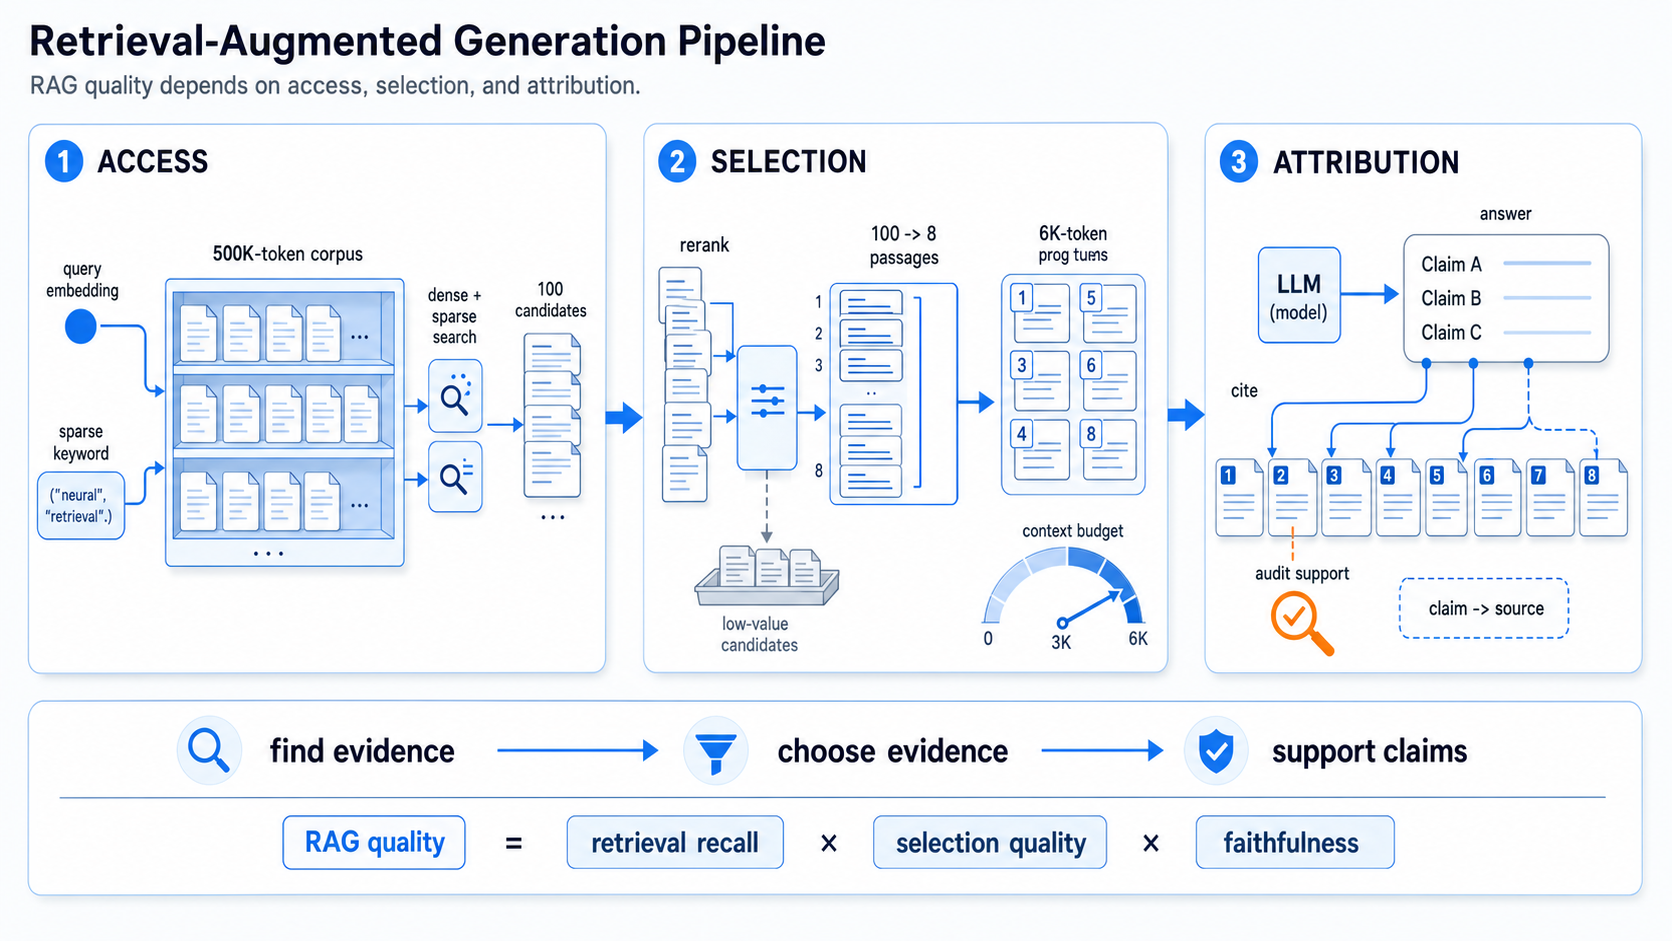
\includegraphics[width=0.96\textwidth]{figures/ch20/fig_rag_attribution_pipeline.png}
\caption{\textbf{RAG as access, selection, and attribution.} Retrieval finds candidate evidence, reranking and packing decide what enters the prompt, generation produces the answer, and citation checking asks whether each claim is supported by the cited source.}
\label{fig:ch20-rag-attribution-pipeline}
\end{figure}

\begin{quickrecap}
\textbf{Quick Recap.}
\begin{itemize}[nosep,leftmargin=1.5em]
  \item RAG is an information access system, not just a vector database.
  \item Access finds candidates; selection decides what enters context; attribution audits generated claims.
  \item Retrieval recall and generation faithfulness are separate bottlenecks.
\end{itemize}
\end{quickrecap}


%----------------------------------------------------------------------
\section{Hybrid Context Systems: RAG, Long Context, Caching, and Routing}
\label{sec:ch20-hybrid-routing}

The frontier is not choosing RAG or long context. The frontier is deciding what to route into the context window.

Li et al.\ compared RAG and long-context LLMs and found a useful pattern: when resourced sufficiently, long-context reading can outperform RAG on average, but RAG has a major cost advantage. Their Self-Route approach asks the model to route queries between RAG and long-context processing to preserve much of the long-context performance while reducing compute cost~\cite{li2024raglongcontext}. The broader design lesson is simple: context path should be conditional on the query.

\subsection{Context Routing Options}

\begin{center}
\begin{tabularx}{\textwidth}{@{}p{0.23\textwidth}p{0.31\textwidth}X@{}}
\toprule
\textbf{Context path} & \textbf{Best fit} & \textbf{Main failure risk} \\
\midrule
Direct answer & Simple question already covered by model or short prompt & Parametric hallucination; no audit trail \\
Read-all long context & Small or medium stable corpus where missing evidence is costly & Attention dilution; stale or contradictory evidence \\
Retrieve-then-read & Large dynamic corpus with local evidence needs & Retrieval miss; ranker chooses hard negatives \\
Cache-then-read & Stable repeated corpus or shared prefix & Cached context becomes stale; access control drift \\
RAG + long reader & Cross-document synthesis or long evidence units & Too much distractor context; attribution becomes harder \\
Agentic search & Open-ended exploration requiring multiple searches or tools & Control-flow errors; loops; tool failures; see Ch21 \\
\bottomrule
\end{tabularx}
\end{center}

The third column matters. A routing decision is also a monitoring decision. If the system chooses RAG, test retrieval recall. If it chooses read-all context, test position sensitivity and distractor robustness. If it chooses caching, test staleness and permission boundaries. If it chooses agentic search, Chapter~\ref{ch:tool-use-agent-loops} will add trace evaluation and tool recovery.

\subsection{LongRAG as a Hybrid Pattern}

LongRAG-style designs show how long context and retrieval can cooperate. Instead of retrieving tiny chunks, the system retrieves longer units, sometimes entire grouped documents, and asks a long-context reader to reason over them~\cite{jiang2024longrag}. The retriever no longer has to locate the exact sentence. The reader no longer has to infer from a context-free snippet.

This is especially relevant for research workflows. A paper's method section, result table, and limitation paragraph may matter together. Chunking them into isolated snippets can break the reasoning chain. A long reader can preserve that chain, but only if the retrieval unit is not so large that irrelevant material overwhelms the evidence.

\subsection{GraphRAG as a Boxed Exception, Not the Main Path}

Some questions are not local. ``What themes recur across all interview transcripts?'' or ``Which teams are central in this incident history?'' may require global structure rather than a few passages. GraphRAG-style systems extract entities, relations, communities, and summaries so that retrieval can operate over a structured representation rather than only raw chunks~\cite{microsoft2026graphrag}. This is worth knowing, but it should not take over the chapter. For this book, GraphRAG is an example of a broader principle: some context systems retrieve \emph{representations of the corpus}, not only text spans.

\begin{tcolorbox}[colback=blue!5, colframe=blue!40, title=\textbf{Is RAG Dead When Context Windows Get Large?}]
No. Large windows reduce the need for brittle short-chunk retrieval in some settings. They do not solve cost, staleness, access control, ranking, or attribution. RAG also evolves: it can retrieve longer units, structured summaries, or cached corpora. The practical question is not ``RAG or long context?'' It is ``which evidence path gives enough coverage, low enough cost, and an answer we can audit?''
\end{tcolorbox}

\begin{figure}[t]
\centering
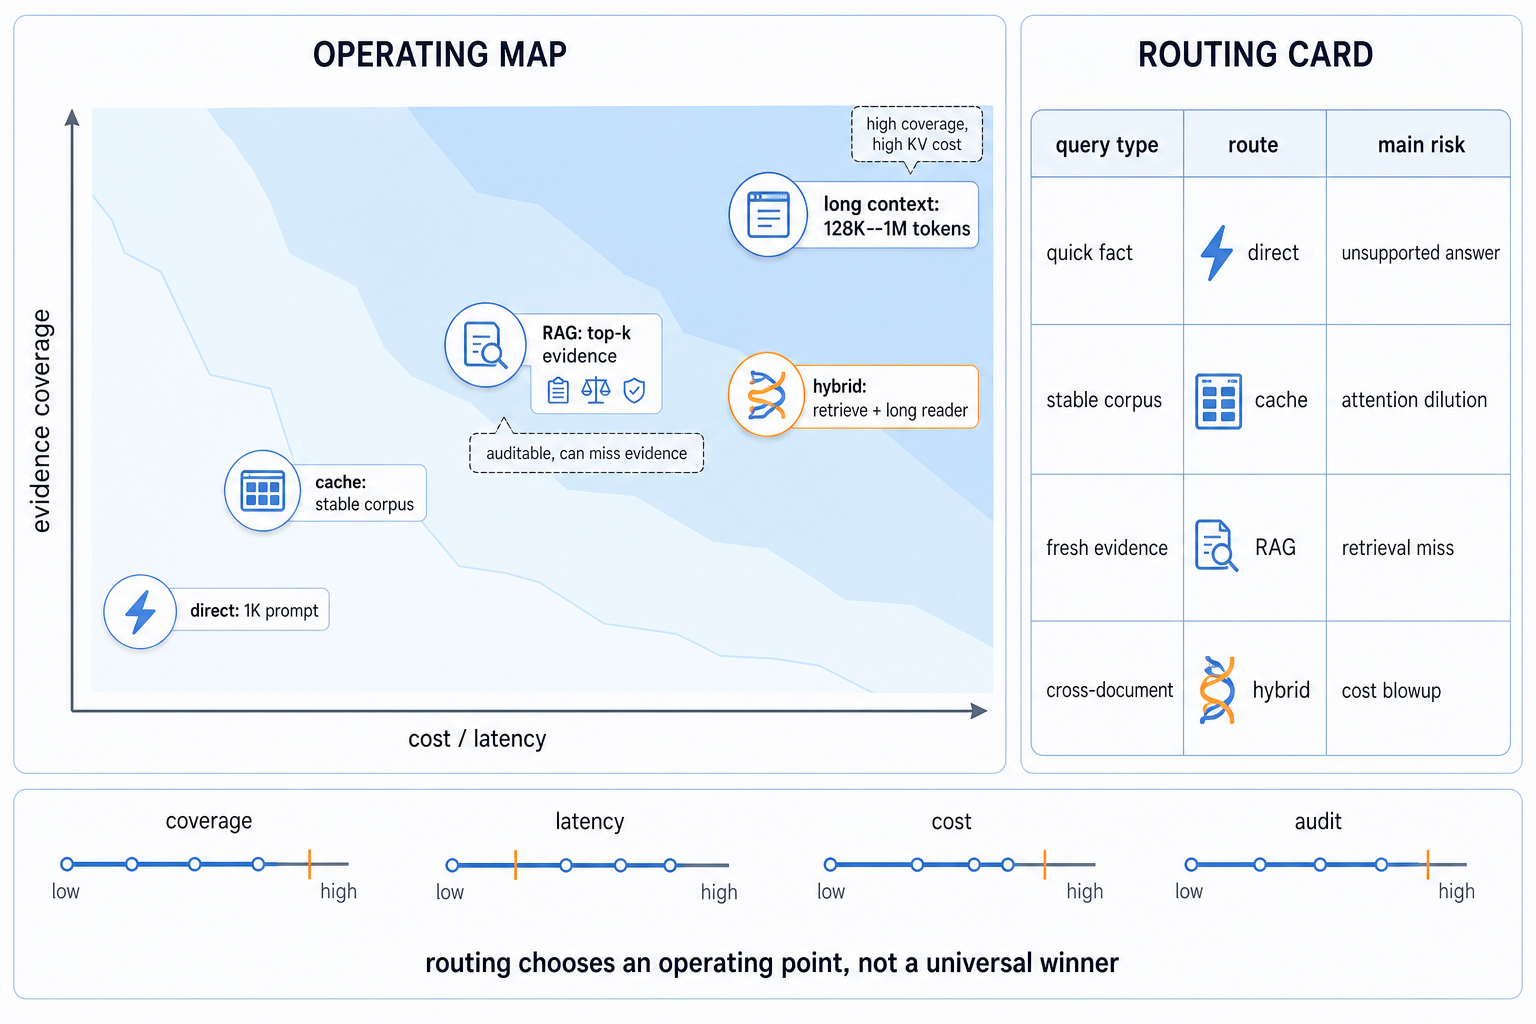
\includegraphics[width=0.96\textwidth]{figures/ch20/fig_context_tradeoff_frontier.png}
\caption{\textbf{Long context, RAG, caching, and hybrid tradeoffs.} Different context paths occupy different regions of the cost, latency, coverage, and auditability space. Routing chooses an operating point for a particular query, not a universal winner.}
\label{fig:ch20-context-tradeoff-frontier}
\end{figure}

\begin{quickrecap}
\textbf{Quick Recap.}
\begin{itemize}[nosep,leftmargin=1.5em]
  \item Hybrid systems route each query to an evidence path.
  \item The routing table should include failure risk, not only expected quality.
  \item Long-context readers and retrieval complement each other when evidence units are longer than snippets.
\end{itemize}
\end{quickrecap}


%----------------------------------------------------------------------
\section{Context Compression and Summarization}
\label{sec:ch20-compression}

When evidence, history, or tool traces exceed the context budget, the system can compress them. Compression is a cost optimization and an information bottleneck. It can reduce latency, fit more history, and make the prompt easier to scan. It can also delete the only detail that matters.

\subsection{Extractive and Abstractive Compression}

\textbf{Extractive compression} keeps selected spans from the original source. It preserves wording and makes citation easier, but it may miss the connective tissue between spans. \textbf{Abstractive compression} rewrites information into a shorter summary. It can combine evidence across sources, but it introduces model judgment and can distort facts.

For the capstone assistant, extractive compression is safer when the user asks for an exact number, code path, or experimental setting. Abstractive compression is useful when the user asks for a narrative summary of a week of work. The system should choose based on the failure cost: exact evidence favors extraction; broad synthesis can tolerate summarization if sources remain available.

\subsection{Hierarchical Summaries}

Long projects often need hierarchical memory: raw documents at the bottom, chunks or sections above them, document summaries above those, and a compact working brief at the top. This mirrors map-reduce summarization. The first pass summarizes local units; later passes combine them into higher-level summaries.

The risk is summary drift. Each layer can drop qualifiers, uncertainty, failed runs, or minority evidence. A good system stores summaries as navigation aids, not as replacements for raw evidence. When a generated answer depends on a summary, the system should still be able to drill back down to source passages.

\subsection{Prompt Compression}

Prompt compression methods try to shorten the visible context while preserving the information needed for the task. In agent systems, compaction can remove old tool outputs, repeated messages, and low-value trace details; Anthropic's discussion of context engineering emphasizes that compaction is a recall-precision tradeoff: aggressive compaction can remove subtle context whose importance appears later~\cite{anthropic2025contextengineering}.

This chapter treats prompt compression as a context mechanism, not an agent-control mechanism. The agent scratchpad and step-by-step state machine come in Chapter~\ref{ch:tool-use-agent-loops}. Here the core question is: what information can be safely shortened without breaking the answer?

\begin{figure}[t]
\centering
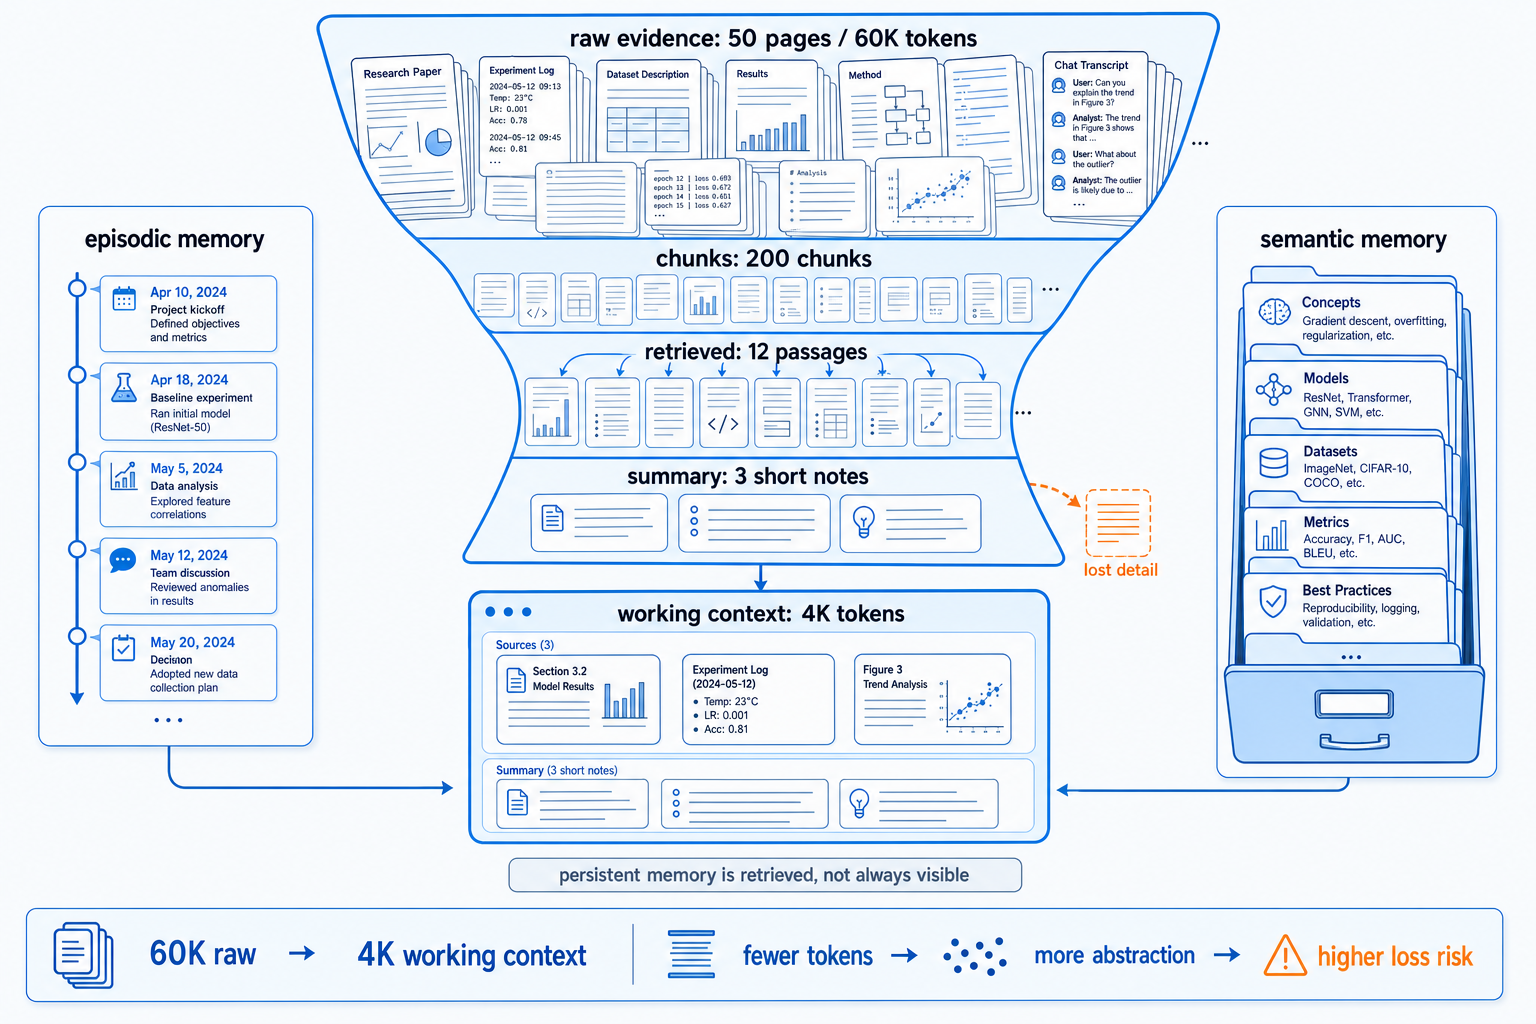
\includegraphics[width=0.96\textwidth]{figures/ch20/fig_compression_memory_hierarchy.png}
\caption{\textbf{Compression and memory hierarchy.} Raw documents can be segmented, retrieved, summarized, packed into working context, or written to persistent memory. Each upward step saves tokens but increases the risk of information loss.}
\label{fig:ch20-compression-memory-hierarchy}
\end{figure}

\begin{center}
\fbox{\begin{minipage}{0.92\textwidth}
\textbf{Pause and Verify.} A system retrieves $12$ passages of $900$ tokens each and has only $6{,}000$ evidence tokens available after system instructions, user query, and output reserve. It can either keep $6$ raw passages or compress all $12$ passages to $450$ tokens each. What failure risk changes? Keeping raw passages may miss evidence in the excluded six. Compressing all passages improves coverage but risks deleting exact numbers, caveats, or source phrasing needed for attribution.
\end{minipage}}
\end{center}

\begin{quickrecap}
\textbf{Quick Recap.}
\begin{itemize}[nosep,leftmargin=1.5em]
  \item Compression trades tokens for information loss risk.
  \item Extractive compression preserves source wording; abstractive compression can synthesize but distort.
  \item Summaries should guide retrieval back to raw evidence, not replace the evidence contract.
\end{itemize}
\end{quickrecap}


%----------------------------------------------------------------------
\section{Memory Across Turns and Sessions}
\label{sec:ch20-memory}

Memory is context that persists beyond the current call. It is not magic, and it is not automatically beneficial. A memory system decides what to write, retrieve, trust, update, and forget.

This section deliberately uses a narrow definition. Agent scratchpads, plans, and step-by-step control state belong to Chapter~\ref{ch:tool-use-agent-loops}. Here, memory means persistent information management across turns, tasks, or sessions.

\subsection{Working, Episodic, and Semantic Memory}

\textbf{Working context} is what the model can currently see in the prompt. It is fast and explicit, but limited by the context budget. \textbf{Episodic memory} stores past events: earlier user requests, experiment runs, decisions, or meetings. \textbf{Semantic memory} stores more stable facts: project definitions, user preferences, dataset descriptions, coding conventions, and long-lived constraints. A fourth category, \textbf{procedural memory}, stores reusable workflows; in this book we mostly leave it to the agent chapter.

The capstone assistant might store that the project uses a specific benchmark split as semantic memory, that a run failed last Friday as episodic memory, and that the current answer is comparing two ablation tables as working context. Mixing these categories causes errors. A failed run should not become a stable fact. A stable safety constraint should not be dropped as disposable conversation history.

\subsection{Write, Retrieve, Update, Forget}

Memory has four basic operations:

\begin{itemize}[nosep]
  \item \textbf{Write}: decide what should persist after the current interaction.
  \item \textbf{Retrieve}: decide which memories are relevant now.
  \item \textbf{Update}: revise old memories when new evidence supersedes them.
  \item \textbf{Forget}: delete or expire information that is obsolete, private, or harmful to retain.
\end{itemize}

Most memory failures are policy failures. The system writes too much, retrieves stale memories, fails to update after correction, or stores sensitive information without a retention reason. More memory is not always better; it increases the surface area for stale context and privacy risk.

\begin{tcolorbox}[colback=orange!5, colframe=orange!60, title=\textbf{For Project~4: Evaluate Memory as Evidence, Not Vibes}]
If you add memory to the Project~4 assistant, log every memory write and retrieval. For each answer, report whether the retrieved memory was necessary, helpful but not necessary, irrelevant, stale, or harmful. Memory should improve task success and auditability, not merely make the assistant sound more personalized.
\end{tcolorbox}

\begin{quickrecap}
\textbf{Quick Recap.}
\begin{itemize}[nosep,leftmargin=1.5em]
  \item Memory is persistent context management, not agent control flow.
  \item Working, episodic, and semantic memory have different update rules.
  \item A memory system needs write, retrieve, update, and forget policies.
\end{itemize}
\end{quickrecap}


%----------------------------------------------------------------------
\section{Failure Modes and Diagnostics}
\label{sec:ch20-failure-diagnostics}

Many context-system failures appear to the user as hallucination. The answer is wrong, unsupported, stale, or overconfident. But the root cause may not be the generator alone. It may be access, selection, packing, compression, memory, or attribution.

\subsection{Failure Taxonomy}

\begin{center}
\begin{tabularx}{\textwidth}{@{}p{0.23\textwidth}X@{}}
\toprule
\textbf{Failure} & \textbf{What went wrong} \\
\midrule
Retrieval miss & The correct evidence was not retrieved at all. \\
Ranking error & Correct evidence was retrieved but ranked below distractors. \\
Packing error & Correct evidence was available but excluded from the final prompt. \\
Context distraction & Irrelevant or hard-negative evidence changed the answer. \\
Position sensitivity & The answer changes when evidence order changes. \\
Summary distortion & Compression removed or altered a necessary detail. \\
Stale memory & Old persistent context overrides newer evidence. \\
Permission mismatch & The system retrieves or exposes evidence the current user should not access. \\
Privacy persistence & The memory store retains sensitive information without a valid reason or expiration policy. \\
Citation mismatch & The cited source is related but does not support the claim. \\
Attribution without support & The answer looks cited but the claim is not entailed by the evidence. \\
\bottomrule
\end{tabularx}
\end{center}

\subsection{Diagnostic Tests}

Good diagnostics isolate the bottleneck:

\begin{itemize}
  \item \textbf{Remove retrieval}: If the answer barely changes when retrieved evidence is removed, retrieval is not contributing.
  \item \textbf{Oracle retrieval}: Give the model the correct evidence. If the answer becomes correct, retrieval or ranking was the bottleneck.
  \item \textbf{Oracle reader}: Ask a simpler model or human to answer from the retrieved evidence. If they can, the generator failed to use the evidence.
  \item \textbf{Shuffle evidence order}: If the answer changes, the system is position-sensitive.
  \item \textbf{Insert distractors}: If plausible but irrelevant passages degrade performance, selection and packing are weak.
  \item \textbf{Citation audit}: Check whether each cited source actually supports each claim.
\end{itemize}

Citation audit should be claim-level, not answer-level. A source attached to the paragraph is not enough; each factual claim should be checked against the specific evidence span that supposedly supports it.

These tests prepare for Chapter~\ref{ch:evaluating-model-systems}. A system benchmark should not only report end-to-end success. It should identify whether failure comes from retrieval, reading, memory, or attribution.

\begin{figure}[t]
\centering
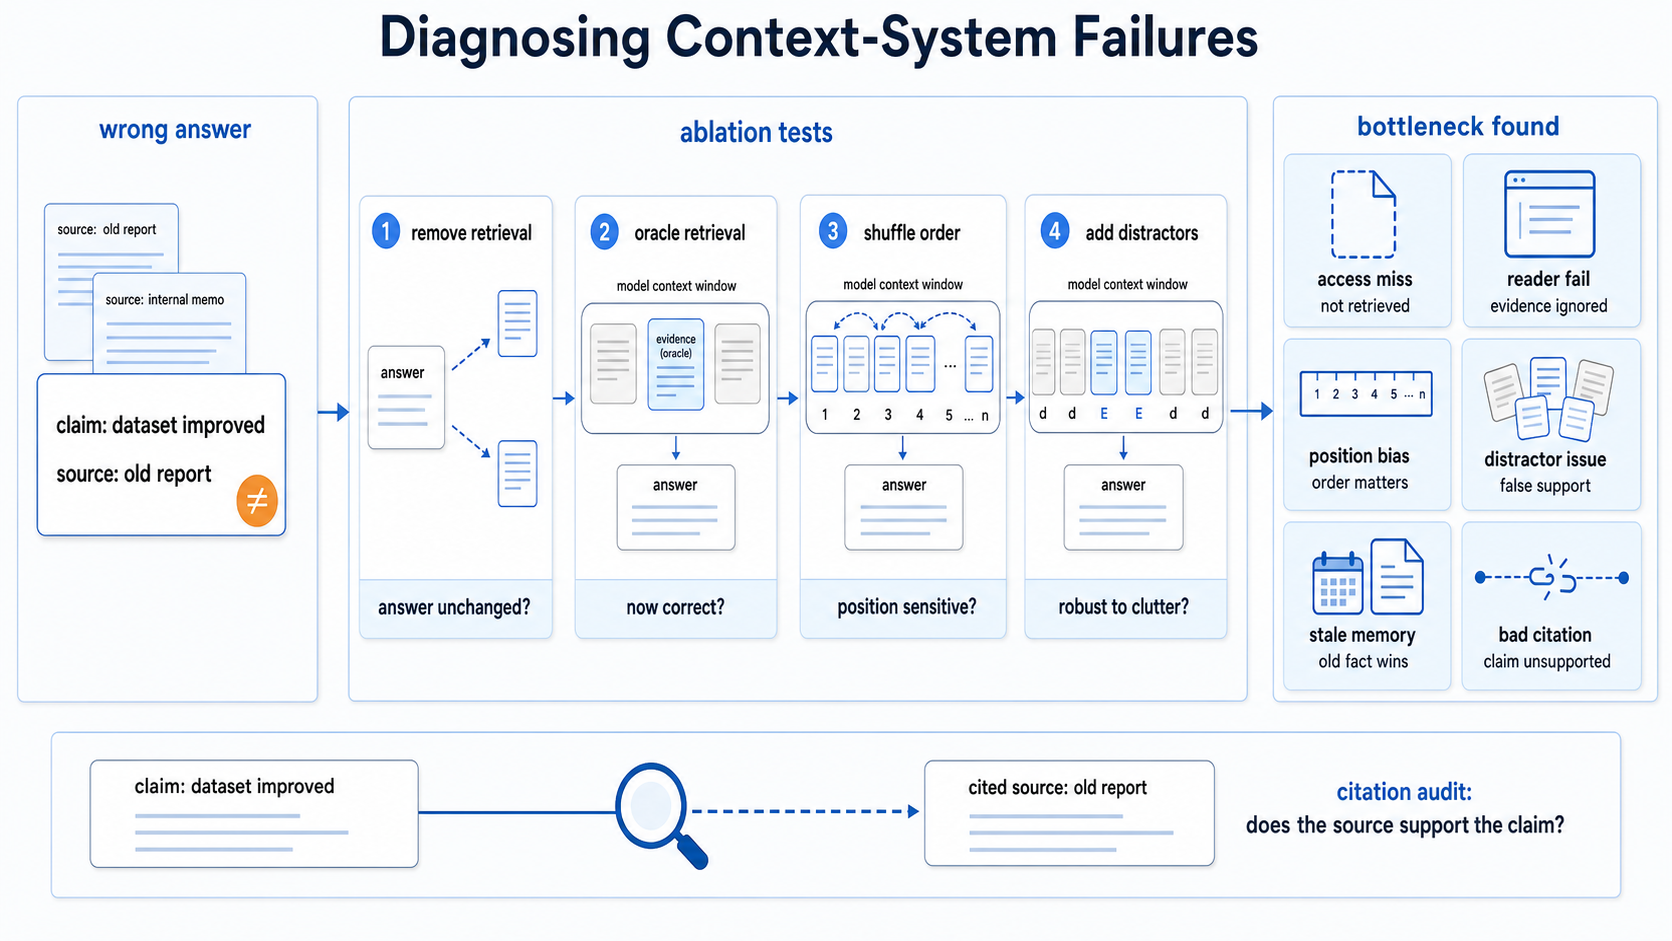
\includegraphics[width=0.96\textwidth]{figures/ch20/fig_diagnostic_decision_tree.png}
\caption{\textbf{Diagnostic decision tree for context failures.} When an answer is wrong, use ablations and oracle conditions to locate the bottleneck: retrieval, reader/generator, position sensitivity, distractor robustness, memory staleness, or citation support.}
\label{fig:ch20-diagnostic-decision-tree}
\end{figure}

\begin{center}
\fbox{\begin{minipage}{0.92\textwidth}
\textbf{Pause and Verify.} Your RAG assistant answers a question incorrectly. With oracle retrieval, it answers correctly. With the original retrieval results shuffled, the answer changes. Which bottlenecks are implicated? Oracle retrieval improving the answer suggests access or selection failed. Sensitivity to shuffling suggests the reader is also position-sensitive. The fix is not only ``use a better generator''; evaluate retrieval recall, reranking, and evidence order.
\end{minipage}}
\end{center}

\begin{quickrecap}
\textbf{Quick Recap.}
\begin{itemize}[nosep,leftmargin=1.5em]
  \item Wrong answers can originate before generation: retrieval, packing, compression, or memory may be at fault.
  \item Oracle and ablation tests separate access failures from reader failures.
  \item Citation audits are necessary because a cited answer is not automatically a claim-supported answer.
\end{itemize}
\end{quickrecap}

\begin{tcolorbox}[colback=orange!5, colframe=orange!60, title=\textbf{For Project~4: Report the Context System}]
For each evaluated assistant, report the context route used: direct, long-context, RAG, cache, compressed, or hybrid. Log retrieved candidates and selected evidence; input tokens spent on evidence, history, and memory; retrieval recall when oracle labels exist; answer success with and without retrieval; claim-level citation support rate; stale or irrelevant memory rate; and the latency/cost measures from Chapter~\ref{ch:serving-quantization-cost}. Project~4 should measure the evidence path, not just the final answer.
\end{tcolorbox}


%----------------------------------------------------------------------
\section{Summary: The Context-as-Runtime Lesson}
\label{sec:ch20-summary}

The main lesson of this chapter is the \textbf{context-as-runtime lesson}: context is a managed substrate, not a passive string. A capable assistant does not simply ask for a larger window or bolt on a vector database. It decides when to read more, when to retrieve, when to cache, when to compress, when to remember, and when to cite.

Long context changes what can fit. Retrieval changes what can be accessed. Caching changes what can be reused cheaply. Compression changes what can fit under a budget. Memory changes what persists across time. Attribution changes whether the answer can be audited. None of these components wins universally. Their value depends on the task, corpus, latency budget, privacy constraints, and failure cost.

For the rest of Part~IV, this chapter supplies the information-access layer. Chapter~\ref{ch:tool-use-agent-loops} will add action: tools, workflows, and agent loops. Chapter~\ref{ch:evaluating-model-systems} will evaluate the full system. A good context system is not judged by how many tokens it stores. It is judged by whether the model sees the right evidence in a form it can use and cite.

\section*{Key Equations}

\begin{center}
\begin{tabularx}{\textwidth}{@{}lX@{}}
\toprule
\textbf{Expression} & \textbf{Interpretation} \\
\midrule
$C_{\text{used}} = C_{\text{system}} + C_{\text{task}} + C_{\text{evidence}} + C_{\text{history}} + C_{\text{output reserve}}$ & Context budget is shared by instructions, task, evidence, history, and room to generate. \\
$R_k(q) = \operatorname{topk}_{d_i \in D} s(q,d_i)$ & Retrieval returns the top-scored evidence units under a scoring function. \\
$E = \operatorname{pack}(R_k(q), C)$ & Context construction packs selected evidence into a finite budget. \\
$A = G(q,E,M)$ & The answer depends on the query, visible evidence, and any retrieved memory. \\
\bottomrule
\end{tabularx}
\end{center}

\section*{Key Checks}

\begin{itemize}
  \item Can you explain why a larger context window can still fail on a long-document question?
  \item Can you separate RAG access, selection, and attribution failures?
  \item Can you choose between direct answering, long-context reading, RAG, caching, and hybrid routing for a concrete query?
  \item Can you describe when compression should keep raw evidence rather than summarize?
  \item Can you distinguish persistent memory from the agent scratchpad of Chapter~\ref{ch:tool-use-agent-loops}?
  \item Can you design an oracle retrieval or citation audit test for a failed answer?
\end{itemize}

\section*{Key Readings}

\begin{itemize}
  \item Lewis et al., ``Retrieval-Augmented Generation for Knowledge-Intensive NLP Tasks''~\cite{lewis2020rag}.
  \item Liu et al., ``Lost in the Middle: How Language Models Use Long Contexts''~\cite{liu2023lost}.
  \item Hsieh et al., ``RULER: What's the Real Context Size of Your Long-Context Language Models?''~\cite{hsieh2024ruler}.
  \item Jiang et al., ``LongRAG: Enhancing Retrieval-Augmented Generation with Long-context LLMs''~\cite{jiang2024longrag}.
  \item Li et al., ``Retrieval Augmented Generation or Long-Context LLMs?''~\cite{li2024raglongcontext}.
  \item Modarressi et al., ``NoLiMa: Long-Context Evaluation Beyond Literal Matching''~\cite{modarressi2025nolima}.
  \item Yuan et al., ``Native Sparse Attention: Hardware-Aligned and Natively Trainable Sparse Attention''~\cite{yuan2025nsa}.
  \item DeepSeek, ``DeepSeek-V4 Preview Release,'' and the Hugging Face DeepSeek-V4-Pro model card~\cite{deepseek2026v4release,deepseek2026v4hf}.
  \item vLLM, ``DeepSeek V4 in vLLM: Efficient Long-Context Attention''~\cite{vllm2026deepseekv4}.
  \item Microsoft Research, ``Project GraphRAG''~\cite{microsoft2026graphrag}.
  \item Google AI for Developers, ``Context Caching''~\cite{google2026contextcaching}.
\end{itemize}
